\documentclass[10pt,a4paper]{article}
\usepackage[utf8]{inputenc}
\usepackage{amsthm, amsmath, mathtools, amssymb}
\usepackage[left=2cm,right=2cm,top=2cm,bottom=2cm]{geometry}
\usepackage[colorlinks,linkcolor=blue,citecolor=blue,urlcolor=blue]{hyperref}
\usepackage[catalan]{babel}
\usepackage{titlesec}
\usepackage{enumitem}
\usepackage{physics}
\usepackage{fancyhdr}
\usepackage{subcaption}

\newcommand{\NN}{\ensuremath{\mathbb{N}}} % set of natural numbers
\newcommand{\ZZ}{\ensuremath{\mathbb{Z}}} % set of integers
\newcommand{\QQ}{\ensuremath{\mathbb{Q}}} % set of rationals
\newcommand{\RR}{\ensuremath{\mathbb{R}}} % set of real numbers
\newcommand{\CC}{\ensuremath{\mathbb{C}}} % set of complex numbers
\newcommand{\KK}{\ensuremath{\mathbb{K}}} % a general field

\newcommand{\vf}[1]{\boldsymbol{\mathrm{#1}}} % math style for vectors and matrices and vector-values functions (previously it was \*vb{#1} but this does not apply to greek letters)
\newcommand{\ii}{\mathrm{i}} % imaginary unit
\renewcommand{\O}[1]{\mathrm{O}\left(#1\right)} % big O-notation

\newtheorem{theorem}{Teorema}
\newtheorem{exercici}{Exercice}
\newtheorem{prop}{Proposició}
\theoremstyle{definition}
\newtheorem{definition}{Definició}
\theoremstyle{remark}
\newtheorem*{res}{Resolution}
\DeclareDocumentCommand\derivative{ s o m g d() }{ 
  % Total derivative
  % s: star for \flatfrac flat derivative
  % o: optional n for nth derivative
  % m: mandatory (x in df/dx)
  % g: optional (f in df/dx)
  % d: long-form d/dx(...)
    \IfBooleanTF{#1}
    {\let\fractype\flatfrac}
    {\let\fractype\frac}
    \IfNoValueTF{#4}
    {
        \IfNoValueTF{#5}
        {\fractype{\diffd \IfNoValueTF{#2}{}{^{#2}}}{\diffd #3\IfNoValueTF{#2}{}{^{#2}}}}
        {\fractype{\diffd \IfNoValueTF{#2}{}{^{#2}}}{\diffd #3\IfNoValueTF{#2}{}{^{#2}}} \argopen(#5\argclose)}
    }
    {\fractype{\diffd \IfNoValueTF{#2}{}{^{#2}} #3}{\diffd #4\IfNoValueTF{#2}{}{^{#2}}}\IfValueT{#5}{(#5)}}
} % differential operator
\DeclareDocumentCommand\partialderivative{ s o m g d() }{ 
  % Total derivative
  % s: star for \flatfrac flat derivative
  % o: optional n for nth derivative
  % m: mandatory (x in df/dx)
  % g: optional (f in df/dx)
  % d: long-form d/dx(...)
  \IfBooleanTF{#1}
    {\let\fractype\flatfrac}
    {\let\fractype\frac}
    \IfNoValueTF{#4}{
      \IfNoValueTF{#5}
      {\fractype{\partial \IfNoValueTF{#2}{}{^{#2}}}{\partial #3\IfNoValueTF{#2}{}{^{#2}}}}
      {\fractype{\partial \IfNoValueTF{#2}{}{^{#2}}}{\partial #3\IfNoValueTF{#2}{}{^{#2}}} \argopen(#5\argclose)}
    }
    {\fractype{\partial \IfNoValueTF{#2}{}{^{#2}} #3}{\partial #4\IfNoValueTF{#2}{}{^{#2}}}\IfValueT{#5}{(#5)}}
} % partial differential operator

\titleformat{\section}
  {\normalfont\fontsize{11}{15}\bfseries}{\thesection}{1em}{}

% \renewcommand{\theenumi}{\textbf{\arabic{enumi}}}
\renewcommand{\theenumi}{\alph{enumi}}
\renewcommand{\theenumiii}{\roman{enumiii}}
\renewcommand{\exp}[1]{\mathrm{e}^{#1}} % exponential function
\DeclareMathOperator*{\im}{Im}
\setlength\multlinegap{0pt} % disable the margins on \begin{multline} command.

\title{\bfseries\Large Diferències finites per a equacions d'evolució}

\author{Víctor Ballester Ribó\\NIU: 1570866}
\date{\parbox{\linewidth}{\centering
  Integració numèrica d'equacions en derivades parcials\endgraf
  Grau en Matemàtiques\endgraf
  Universitat Autònoma de Barcelona\endgraf
  Juny de 2023}}
  \pagestyle{fancy}
  \fancyhf{}
  \fancyhfoffset[L]{1cm}
  \fancyhfoffset[R]{1cm}
  \rhead{NIU: 1570866}
  \lhead{Víctor Ballester}
  \cfoot{\thepage}
  %\setlength{\headheight}{13.6pt}

\setlength{\parindent}{0pt}
\begin{document}
\selectlanguage{catalan}
\maketitle
L'objectiu d'aquesta pràctica és resoldre el problema mixt següent per a l'equació de la calor en una placa rectangular:
\begin{equation}\label{eq:problema}
  \begin{cases}
    u_t-\Delta u = f & \text{a } [0,T]\times\Omega         \\
    u=g              & \text{a } [0,T]\times\partial\Omega \\
    u=h              & \text{a } \{0\}\times \Omega
  \end{cases}
\end{equation}
on $\Omega$ és la regió rectangular de la placa, que en el nostre cas serà $\Omega = [0,1]\times[0,1]$, i $T$ és el temps final de la simulació.

Donades funcions $f(t,x,y)$, $g(t,x,y)$ i $h(x,y)$ resoldrem aquest problema usant diferències finites. Discretitzem primer l'espai i el temps. Considerem dues particions de l'interval $[0,1]$ en $n_x+1$ i $n_y+1$ subintervals equidistants amb separacions $\delta_x=1/n_x$ i $\delta_y=1/n_y$ respectivament. A més discretitzem l'interval temporal $[0,T]$ en $n_t+1$ subintervals equidistants amb separació $\delta_t=T/n_t$. D'ara endavant, denotarem la solució $u(k\delta_t, i\delta_x, j\delta_y)$ per $u_{k,i,j}$ i les seves respectives aproximacions per diferències finites per $v_{k,i,j}$.

Considerem primer el següent mètode explícit, que s'obté de prendre diferències centrades de segon ordre per l'espai i de primer ordre endavant per al temps:
$$
  v_{k+1,i,j} = (1-2\mu_x - 2\mu_y) v_{k,i,j} + \mu_x (v_{k,i+1,j} + v_{k,i-1,j}) + \mu_y (v_{k,i,j+1} + v_{k,i,j-1}) + \delta_t f_{k,i,j}
$$
on $\mu_x = \delta_t/{\delta_x}^2$ i $\mu_y = \delta_t/{\delta_y}^2$ i $f_{k,i,j}=f(k\delta_t, i\delta_x, j\delta_y)$. Aquest mètode és consistent i estable si $1- 2\mu_x -2 \mu_y \geq 0$. A més, l'error de convergència és $\O{\delta_t + \delta_x^2 + \delta_y^2}$.

Fixem-nos que aquest mètode és exacte per a polinomis de grau $\leq 1$ en $t$ i grau $\leq 3$ en l'espai. Això es deu a l'expansió en sèrie de Taylor de $u$: d'una banda el coeficient que multiplica l'error $\O{\delta_t}$ de la diferència finita pel temps de primer ordre involucra $u_{tt}=0$ i anàlogament amb les derivades centrades per l'espai. Això ho podem comprovar també numèricament. Considerem el polinomi
$$u(t,x,y)=1+t+x^2+y^2+x^3$$
Prenent $f(t,x,y)= -3-6x$, $g(t,x,y)=1+t+x^2+y^2+x^3$ i $h(x,y)=1+x^2+y^2+x^3$ tenim que la solució del problema \eqref{eq:problema} és precisament $u(t,x,y)$. Així doncs, si prenem per exemple $\delta_x=0.1$, $\delta_y=0.1$ i $\delta_t=0.001$, que compleixen la condició d'estabilitat, per a $\Omega = [0,1]\times[0,1]$ i $T=0.1$ obtenim un error en norma $\norm{\cdot}_\infty$ entre la solució real i l'aproximada de $5.77316\cdot 10^{-15}$, que es pot considerar com a error d'aritmètica en punt flotant.\vspace*{0.25cm}

Considerem ara una placa d'acer de densitat $\rho= 7.8\ \frac{\mathrm{g}}{\mathrm{cm}^3}$, conductivitat tèrmica $\kappa = 0.13\ \frac{\mathrm{cal}}{\mathrm{cm}\cdot\mathrm{s}\cdot\mathrm{K}}$ i calor específic $c=0.11\ \frac{\mathrm{cal}}{\mathrm{g}\cdot\mathrm{K}}$. Posem una font de calor a sota de la placa que genera $F(\tau, x,y) \ \frac{\mathrm{cal}}{\mathrm{s}\cdot\mathrm{cm}^3}$ a l'instant $\tau$ i al punt $(x,y)$, on $F$ està definida per:
$$
  F(\tau, x,y) = \begin{cases}
    100 & \text{si } \norm{(x,y)-(\frac{1}{2},\frac{1}{2})}_2 <\frac{1}{5} \\
    0   & \text{altrament}
  \end{cases}
$$
Suposem també que en l'instant $\tau=0$, la placa està a temperatura $0\ ^\circ\mathrm{C}$ i per a tot temps $\tau$ la frontera de la placa es manté també a $0\ ^\circ\mathrm{C}$. En aquestes condicions, l'evolució de la temperatura sobre la placa ve donada per la solució per la solució del següent problema mixt:
$$
  \begin{cases}
    c\rho v_{\tau} -\kappa \Delta v = F(\tau,x,y) & \text{a } [0,T] \times \Omega         \\
    v=0                                           & \text{a } [0,T] \times \partial\Omega \\
    v=0                                           & \text{a } \{0\} \times \Omega         \\
  \end{cases}
$$
Usant el canvi de variables $t=\frac{\kappa}{c\rho}\tau$, tenim que $\dv{t}{\tau}= \frac{\kappa}{c\rho}$ i per tant si $u(t,x,y)=v(\tau,x,y)$, usant la regla de la cadena, $u_t = v_\tau \frac{\kappa}{c\rho}$ (i clarament $\Delta u=\Delta v$). Així doncs, el problema anterior es pot reescriure com:
$$
  \begin{cases}
    \displaystyle u_t -\Delta u = \frac{1}{\kappa} F\left(\frac{c\rho}{\kappa}t,x,y\right) & \displaystyle\text{a } \left[0,\frac{\kappa}{c\rho}T\right] \times \Omega  \vspace{0.1cm} \\
    u=0                                                                                    & \displaystyle\text{a } \left[0,\frac{\kappa}{c\rho}T\right] \times \partial\Omega         \\
    u=0                                                                                    & \text{a } \{0\} \times \Omega                                                             \\
  \end{cases}
$$

La condició d'estabilitat en l'esquema explícit que hem descrit anteriorment és necessària. Fem un experiment numèric per veure què podem obtenir si no se satisfà aquesta condició. Per fer-ho prenem $\delta_x=\delta_y=\delta_t=0.1$ i $T=1$. Amb aquests paràmetres obtenim que en $\tau=0.9$ i la temperatura en la regió de la placa amb $x=0.3$ és:
\begin{table}[ht]
  \centering
  \begin{tabular}{c|c|c}
    $x$ & $y$ & $v(0.9,x,y)$        \\ \hline\hline
    0.3 & 0.0 & 0                   \\
    0.3 & 0.1 & 42286728.810146     \\
    0.3 & 0.2 & $-111988126.131011$ \\
    0.3 & 0.3 & 199241046.679864    \\
    0.3 & 0.4 & $-259680534.657868$ \\
    0.3 & 0.5 & 263234236.257432    \\
    0.3 & 0.6 & $-210322365.754957$ \\
    0.3 & 0.7 & 126199592.465624    \\
    0.3 & 0.8 & $-54636211.331768$  \\
    0.3 & 0.9 & 16318289.975168     \\
    0.3 & 1.0 & 0                   \\
  \end{tabular}
\end{table}
Observem valors molt grossos i negatius, que no tenen sentit físic, ja que estan fora de l'interval $[0,100]$.
El problema d'aquest mètode explícit és que requereix d'un cost elevat computacionalment quan volem els resultats amb una precisió raonable. Per exemple, si volem que $\O{\delta_t + {\delta_x}^2 + {\delta_y}^2} = \O{10^{-4}}$ aleshores podem prendre $\delta_x= \delta_y=0.01$ i $\delta_t=10^{-5}$. D'aquesta manera, $1-2\mu_x-2\mu_y = 0.6>0$ i per tant el mètode és estable. Ara bé, per arribar fins a $\tau=1$ necessitem emprar molt de temps. A la taula següent mostrem el temps que triga el programa a calcular els valors de la temperatura en els punts de la placa fins a diferents temps finals:
\begin{table}[ht]
  \centering
  \begin{tabular}{c|c}
    $T$    & Temps emprat [s] \\ \hline\hline
    0.0001 & 0.047858         \\
    0.001  & 0.569544         \\
    0.01   & 5.613888         \\
    0.1    & 57.489433        \\
  \end{tabular}
  \caption{Temps que triga l'esquema explícit en calcular i escriure a un fitxer tots els valors en cada graella (usant $\delta_x= \delta_y=0.01$ i $\delta_t=10^{-5}$) fins a diferents temps finals.}
\end{table}
Aproximadament cada temps em multiplica per 10 respecte al temps anterior. Per tant, calculem que trigaríem de l'ordre de 5 min per calcular els valors de la temperatura fins a $\tau=1$.\vspace{0.25cm}

Una solució alternativa és emprar un mètode implícit, com ara el de Crank-Nicolson:
\begin{align*}
  \frac{v_{k+1,i,j}-v_{k,i,j}}{\delta_t} & - \frac{1}{2}\left(\frac{v_{k+1,i+1,j}-2v_{k+1,i,j}+v_{k+1,i-1,j}}{{\delta_x}^2} +\frac{v_{k,i+1,j}-2v_{k,i,j}+v_{k,i-1,j}}{{\delta_x}^2} \right)  -                                             \\
                                         & -\frac{1}{2}\left( \frac{v_{k+1,i,j+1}-2v_{k+1,i,j}+v_{k+1,i,j-1}}{{\delta_y}^2}+ \frac{v_{k,i,j+1}-2v_{k,i,j}+v_{k,i,j-1}}{{\delta_y}^2}\right) = \frac{1}{2}\left(f_{k+1,i,j}+f_{k,i,j}\right)
\end{align*}
on hem usat la notació de \eqref{eq:problema}. Per resoldre aquest sistema, hem de resoldre un sistema lineal en les incògnites $\{v_{k+1,i,j}\}_{i,j}$, i usarem el mètode SOR per a fer-ho.

Ara, però, a diferència del que teníem amb el mètode explícit, l'esquema de diferències finites no serà exacte quan l'apliquem a polinomis. En efecte, prenent els mateixos valors que anteriorment ($\delta_x=\delta_y=0.1$, $\delta_t=0.001$ i $T=1$), obtenim un error en norma $\norm{\cdot}_\infty$ de $9.17816\times 10^{-5}$, que està lluny de ser considerat com a errors de punt flotant.

Tot i això, aquest mètode ens permet obtenir una precisió molt més elevada en un temps raonable ja que no tenim cap condició d'estabilitat a satisfer-se i a més l'ordre de convergència és $\O{{\delta_t}^2 + {\delta_x}^2 + {\delta_y}^2}$. A la taula següent mostrem el temps que triga el programa a calcular els valors de la temperatura en els punts de la placa fins a diferents temps finals:
\begin{table}[ht]
  \centering
  \begin{tabular}{c|c}
    $T$  & Temps emprat [s] \\ \hline\hline
    0.01 & 0.111025         \\
    0.1  & 1.057527         \\
    1    & 9.849696
  \end{tabular}
  \caption{Temps que triga l'esquema explícit en calcular i escriure a un fitxer tots els valors en cada graella (usant $\delta_x= \delta_y=0.01$ i $\delta_t=0.001$) fins a diferents temps finals.}
\end{table}
Finalment, donant aquest esquema com a bo, els resultats que obtenim en integrar l'equació de la calor sobre la placa d'acer es mostren a les següents imatges:
\begin{figure}[ht]
  \centering\vspace{-1cm}
  \begin{subfigure}{0.49\linewidth}
    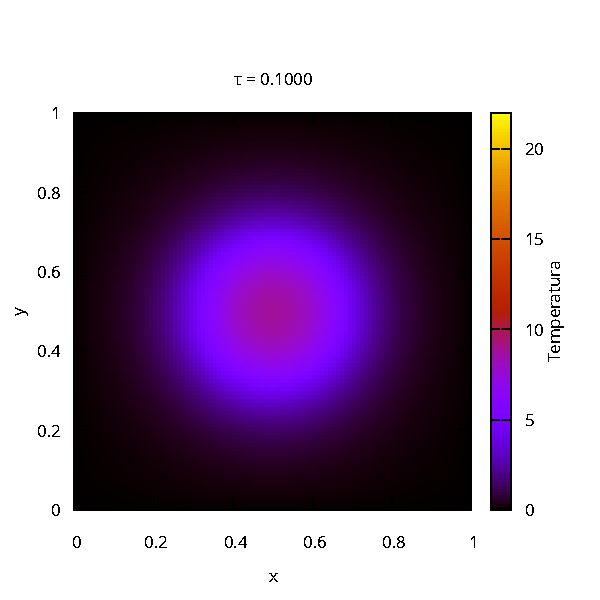
\includegraphics[width=\textwidth]{../plot/Images/heatmap_00010.pdf}
  \end{subfigure}\hfill
  \begin{subfigure}{0.49\linewidth}
    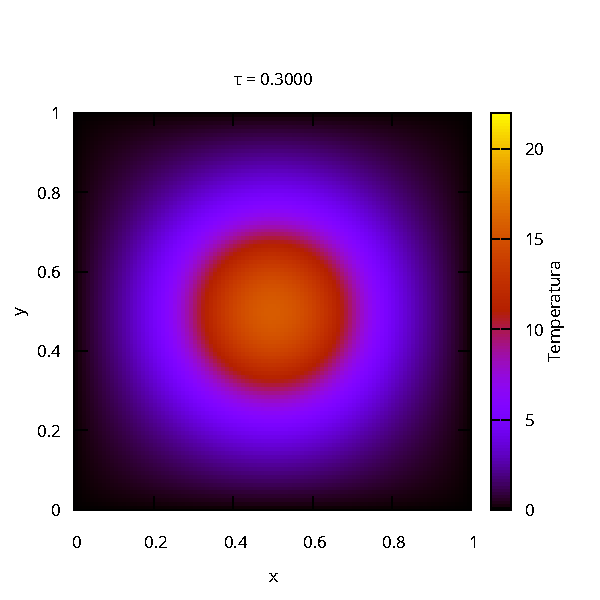
\includegraphics[width=\textwidth]{../plot/Images/heatmap_00030.pdf}
  \end{subfigure}\\\vspace{-1cm}
  \begin{subfigure}{0.49\linewidth}
    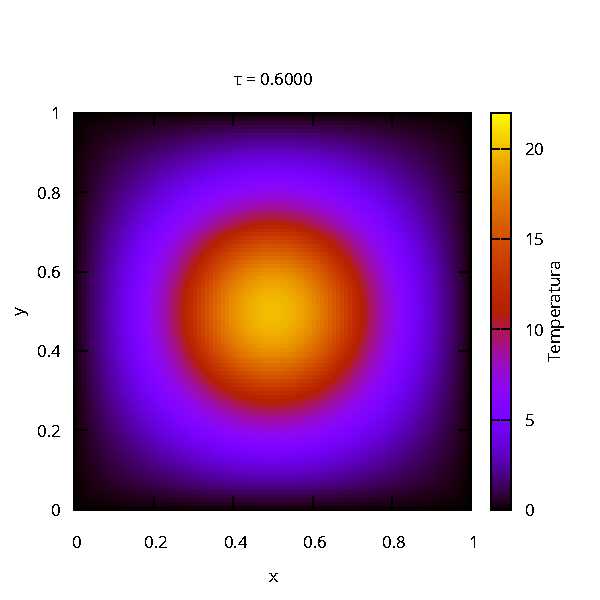
\includegraphics[width=\textwidth]{../plot/Images/heatmap_00060.pdf}
  \end{subfigure}\hfill
  \begin{subfigure}{0.49\linewidth}
    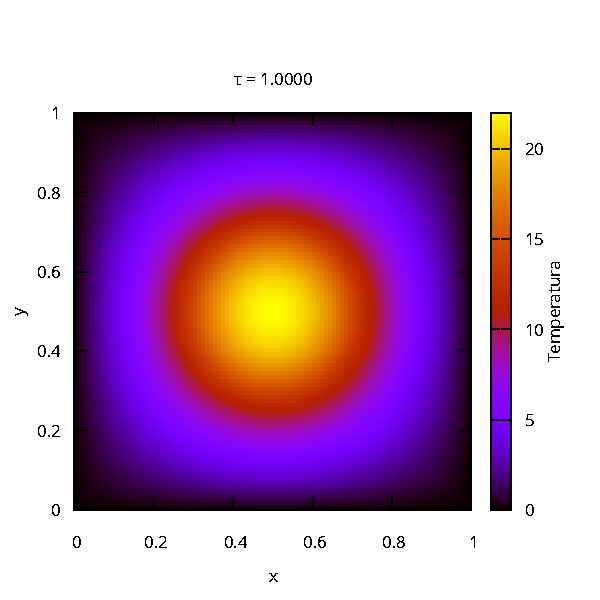
\includegraphics[width=\textwidth]{../plot/Images/heatmap_00100.pdf}
  \end{subfigure}
  \caption{Temperatura a la placa d'acer en els temps $\tau=0.1,0.3,0.6,1$.}
\end{figure}
\begin{figure}[ht]
  \centering
  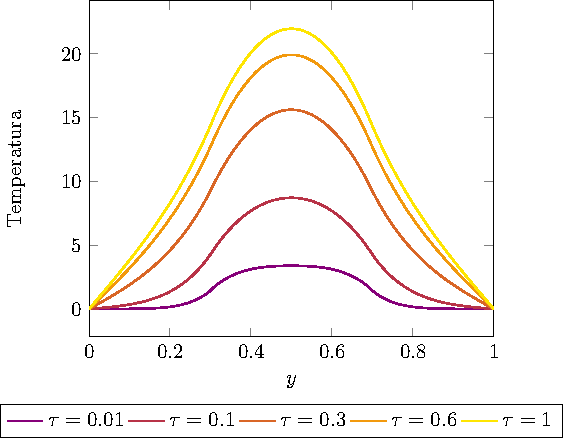
\includegraphics[width=0.5\linewidth]{Images/graphic.pdf}
  \caption{Evolució de la temperatura a la secció $x=0.5$ de la placa.}
\end{figure}
\end{document}